\begin{frame}{Experimental setup}
  \framesubtitle{EXPERIMENT}
  \vspace{-0.08cm}
  \begin{columns}[T,onlytextwidth]
    \begin{column}{0.52\textwidth}
      \begin{align*}
        k &= 10, & q_*(a) &\sim \mathcal{N}(0,1),\\[-0.05cm]
        R_t\mid A_t=a &\sim \mathcal{N}\!\left(q_*(a),1\right).
      \end{align*}
      \vspace{-0.12cm}
      \flatbox{
        \textbf{Fixed testbed, seed 5.} The optimal arm is
        \(a_*=2\) in Python indexing (the third arm), with
        \(q_*(a_*)=2.4308\).
      }
      \vspace{0.15cm}
      \metric{$T=10^4$}{Q4--Q7 horizon}\hfill
      \metric{$M=300$}{independent reruns}
      \vspace{0.10cm}
      \micro{Q3 growth diagnostics extend to \(T=10^5\) with \(M=500\). The same fixed \(q_*\) is used throughout.}
    \end{column}
    \begin{column}{0.44\textwidth}
      \centering
      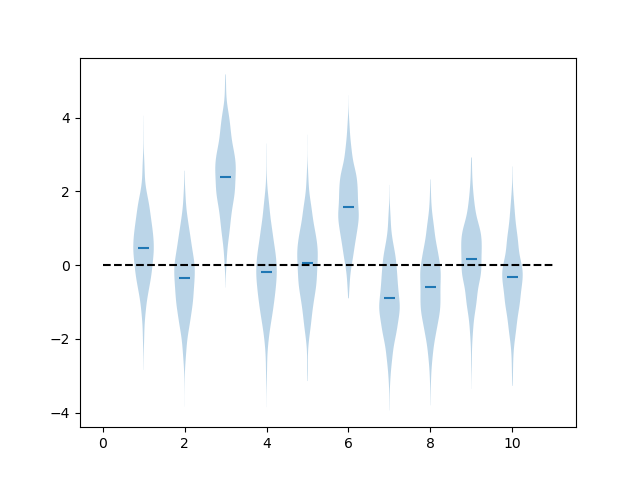
\includegraphics[width=0.92\linewidth]{arms.png}
      \vspace{-0.06cm}
      \smallnote{The simulator knows \(q_*\) only to evaluate pseudo-regret; the agents do not observe it.}
    \end{column}
  \end{columns}
\end{frame}
